\documentclass[12pt]{article}

\usepackage{sbc-template}
\usepackage{graphicx,url}
\usepackage{indentfirst}
\usepackage{listings}
\usepackage{authblk}
\usepackage[utf8]{inputenc}
\usepackage[brazil]{babel}

\title{Comparação de Ferramentas de IA para otimização de instruções SQL}

\address{Centro de Ciências Exatas (CCE) -- Universidade Estadual de Londrina (UEL)\\
  Caixa Postal 10.011 -- 86057-970 -- Londrina -- PR -- Brazil}

\author{Fábio Silva Garbin\inst{1}, Daniel dos Santos Kaster\inst{1} }

\begin{document} 
\pagenumbering{arabic} % Arabic/Indic page numbers
\maketitle

\begin{abstract}
Databases are an important part in software development area and
the time to data access is a critical point in the software performance. In this
study, Our approach is to compare artificial intelligence for generic purpose tools (ChatGPT and Bard) for optimize
database queries.
\end{abstract}
     
\begin{resumo} 
Banco de dados são uma parte importante no desenvolvimento de
software e o tempo de acesso a dados é um fator cada vez mais relevante na
performance dos softwares. Este estudo visa comparar o uso de ferramentas
de inteligência artificial (IA) de propósito genérico para a otimização de
consultas a banco de dados.
\end{resumo}


\section{Introdução}
A velocidade ao acesso a dados fica cada dia mais importante devido a quantidade de
serviços e usuários que desejam ter a informação confiável e disponível no menor
espaço de tempo possível. Os bancos de dados são parte essencial nessa equação
durante o desenvolvimento de softwares.

A consulta aos bancos de dados (\emph{querys}) é a principal maneira de recuperar esses dados de
forma que qualquer otimização em sua execução pode colaborar a obter os dados de
forma mais eficiente trazendo benefícios ao software em questão e também aos
usuários.

As ferramentas de IA estão em constante evolução e podem ser uma opção para ajudar na otimização das \emph{querys} criadas no processo de desenvolvimento de software, este artigo busca avaliar como essas ferramentas (ChatGPT e Bard) de IA podem ajudar neste processo de melhoria da consultas.

O uso de IA na otimização de consultas pode ser aplicado em caso específicos como na ordem de JOINs no plano de execução sugeridas por \cite{robinson2014cost}.

Neste cenário temos a opção de utilizar as ferramentas de forma descritiva com uma abordagem de Text-to-SQL (Texto para SQL) onde é fornecido uma questão em linguagem natural e é gerado como resultado um código SQL para resultar a consulta \cite{li2023can}. O comparativo realizado por \cite{linkedin_compare_texttosql} mostra resultados deste modelo de geração/otimização de consultas SQL ou ainda alguns testes da geração de consultas através de text como em \cite{devblogs_microsoft}.

Em uma segunda visão temos diversas consultas escritas em softwares existentes e neste sentido temos um cenário SQL-to-SQL, onde o dado de entrada é um código de consulta SQL e o retorno é uma código SQL otimizado e/ou sugestões para melhor desempenho da consulta.

Este artigo explora o segundo cenário, SQL-to-SQL, de forma a comparar se as ferramentas de IA de propósito genérico podem colaborar no processo de otimização de consultas SQL.

\section{Método Proposto}

Para realizar essa pesquisa foi selecionado o Sistema de Gerenciador de Banco de Dados (SGBD) PostgresSQL 15 e um dataset público para realizar os testes com as ferrametas de IA selecionadas, ChatGPT e Bard. O banco de dados do IMDb (Internet Movie Database) \cite{developer_imdb} foi o escolhido por apresentar uma quantidade representativa de dados e de fácil acesso.

O método proposto foi divido em 8 etapas:

\begin{enumerate}
  \item Definir e executar a \emph{query}
  \item Executar o opção de Explain
  \item Submeter a \emph{query} as ferramentas de IA ChatGPT e Bard
  \item Aplicar alterações na \emph{query} e/ou estrutura, caso necessário
  \item Executar a nova \emph{query} com as modificações sugeridas pelas ferramentas do IA
  \item Executar o opção de Explain
  \item Comparar resultado o explain
  \item Voltar BD ao estado original
\end{enumerate}

\subsection{Etapas do método}

\subsubsection{Definir e executar a \emph{query}}

Definir \emph{querys} de diferentes complexidades de forma a abranger um maior número de possibilidades de avaliação das ferramentas de IA. A complexidade foi definida utilizando como referência \cite{subali2018new}, quanto maior o valor mais complexa a \emph{query}. Executar a \emph{query} para obter o resultado de forma a validar as modificações sugeridas pelas ferramentas.

\subsubsection{Executar o opção de Explain}

O SGBD PostgreSQL possui a funcionalidade de EXPLAIN \cite{postgresql_explain} que mostra o plano de execução de uma \emph{query}, assim podemos comparar e avaliar as diferenças dos planos de execução entre a \emph{query} original e a modificada pelas ferramentas de IA. 
Dentre as informações fornecidas pela opção EXPLAIN para base comparativa será utilizada o dado de Total Cost, que segundo a documentação indica as unidades de custos (\emph{unit costs}) para retorno de todas as linhas da consulta ou parte dela em questão.

\subsubsection{Submeter a \emph{query} as ferramentas de IA ChatGPT e Bard}

Submeter, manualmente, a \emph{query} nas ferramentas de IA e avaliar as respostas fornecidas, mais de uma iteração com a ferramenta pode ser necessária conforme as respostas fornecidas.

Na execução desta etapa da análise submetemos a \emph{query} as ferramentas ChatGPT e Bard com o mesmo conteúdo no seguinte formato:

\begin{lstlisting}
Como melhorar a \emph{query}: <query>

Com o Schema: <schema do banco de dados IMDB>
\end{lstlisting}

Esse formato foi definido pois com a entrada apenas da \emph{query} as ferramentas trazem respostas genéricas sem uma análise de contexto do banco de dados que está sendo analisado, o que não está no escopo deste trabalho.

\subsubsection{Aplicar alterações na \emph{query} e/ou estrutura, caso necessário}

Realizar alterações na \emph{query} e/ou estrutura do SGBD para atender as sugestões fornecidas pelas ferramentas de IA.

\subsubsection{Executar a nova \emph{query} com as modificações sugeridas pelas ferramentas do IA}

Executar a \emph{query} modificada pelas ferramentas de IA para validar se obtemos o mesmo resultado da \emph{query} inicial.

\subsubsection{Executar o opção de Explain}

Executar a opção de explain com a nova \emph{query} para comparativo com a \emph{query} inicial

\subsubsection{Comparar resultado o explain}

Comparar os planos de execução da \emph{query} inicial e alterada.

\subsubsection{Voltar BD ao estado original}

Para uma análise independente de cada \emph{query} o banco de dados será restaurado ao estado original antes das modificações.

\clearpage
\section{Diagrama de Entidade e Relacionamento (DER)}

O Diagrama de Entidade e Relacionamento (DER) do banco de dado IMDB utilizado inicial pode ser verificado na figura 1.

\begin{figure}[ht]
\centering
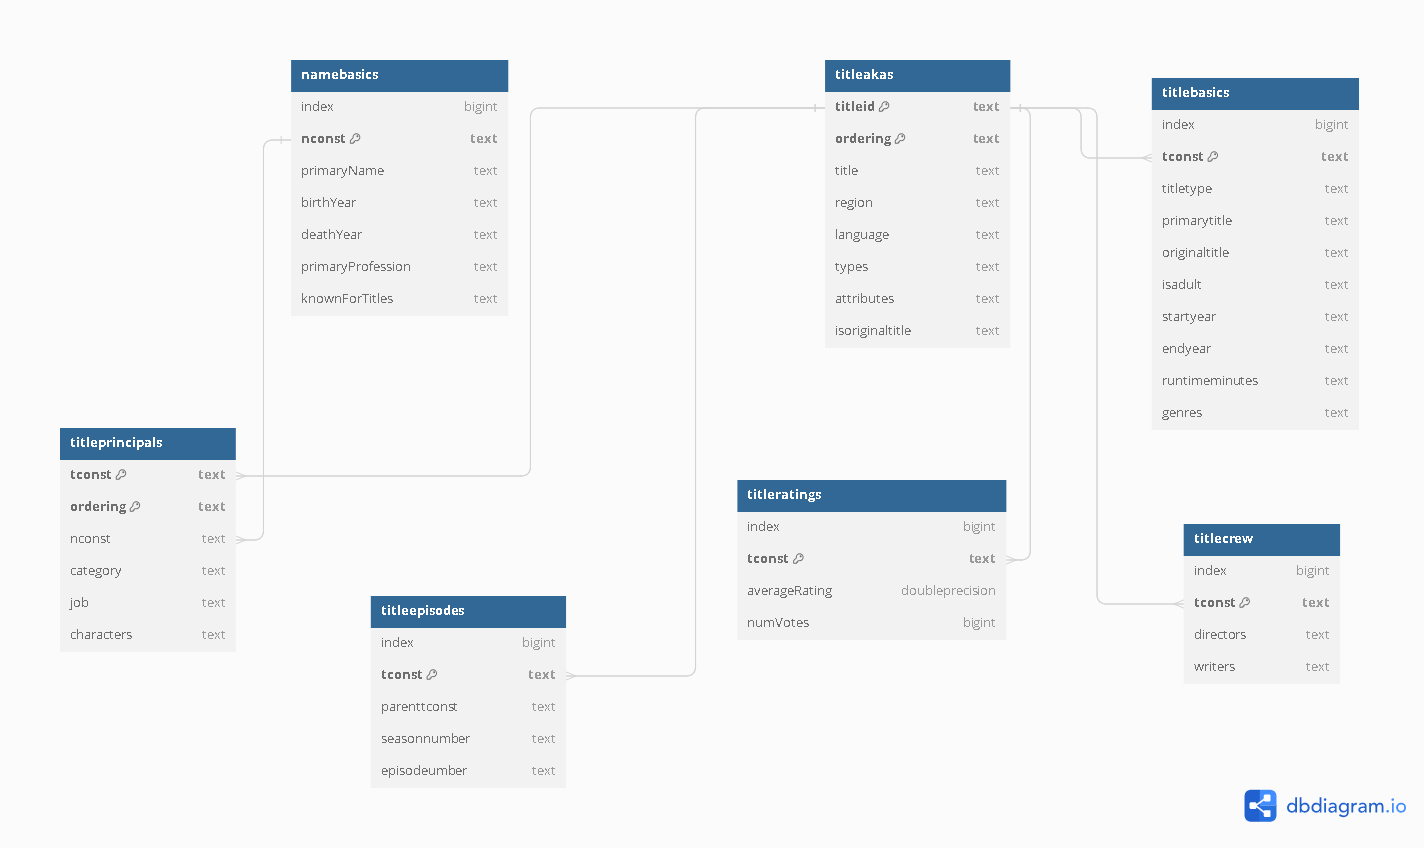
\includegraphics[width=.5\textwidth]{IMDB_DER.png}
\caption{Diagrama de Entidade e Relacionamento (DER) inicial}
\end{figure}

\section{Análise de Consultas}

\subsection{\emph{Query} 01}

A primeira análise, \emph{query} 01, com complexidade de 1.79, realizada foi com a consulta a seguir:

\begin{lstlisting}[language=SQL, caption=\emph{Query} 01]
SELECT titlebasics.tconst
	,titleprincipals.tconst
	,titleprincipals.nconst
	,namebasics.primaryname
FROM titlebasics
INNER JOIN titleprincipals ON 
    titlebasics.tconst = titleprincipals.tconst
INNER JOIN namebasics ON 
titleprincipals.nconst = namebasics.nconst
WHERE titlebasics.tconst = 'tt0075148'
\end{lstlisting}

Na execução inicia da \emph{query} 01 temos um resultado de 10 linhas do banco de dados IMDB agrupando as tabelas titlebasics, titleprincipals e namebasics.

No plano de execução inicial, resumido,  desta consulta temos:
\begin{lstlisting}[breaklines, tabsize=2]
"Plan": {
  "Node Type": "Nested Loop",
  "Join Type": "Inner",
  "Total Cost": 1523838.48,
  "Plans": [
	{
	  "Node Type": "Gather",
	  "Parent Relationship": "Outer",
	  "Total Cost": 216704.46,
	  "Plans": [
		{
		  "Node Type": "Seq Scan",
		  "Parent Relationship": "Outer",
		  "Relation Name": "titlebasics",
		  "Alias": "titlebasics",
		  "Total Cost": 215704.36,
		  "Filter": "(tconst = 'tt0075148'::text)"
		}
	  ]
	},
	{
	  "Node Type": "Gather",
	  "Parent Relationship": "Inner",
	  "Total Cost": 1307132.57,
	  "Plans": [
		{
		  "Node Type": "Hash Join",
		  "Parent Relationship": "Outer",
		  "Join Type": "Inner",
		  "Total Cost": 1306118.07,
		  "Hash Cond": "(titleprincipals.nconst = namebasics.nconst)",
		  "Plans": [
			{
			  "Node Type": "Seq Scan",
			  "Parent Relationship": "Outer",
			  "Relation Name": "titleprincipals",
			  "Alias": "titleprincipals",
			  "Total Cost": 970465.13,
			  "Filter": "(tconst = 'tt0075148'::text)"
			},
			{
			  "Node Type": "Hash",
			  "Parent Relationship": "Inner",
			  "Total Cost": 204549.63,
			  "Plans": [
				{
				  "Node Type": "Seq Scan",
				  "Parent Relationship": "Outer",
				  "Relation Name": "namebasics",
				  "Alias": "namebasics",
				  "Total Cost": 204549.63,
				}
			  ]
			}
		  ]
		}
	  ]
	}
  ]
}
\end{lstlisting}

Após a entrada dos dados as ferramentas trouxeram os seguintes resultados.

Na primeira iteração com as ferramentas ambas sugeriram alterações na formatação e o uso de alias para melhorar a legibilidade do código da consulta e também o uso de índices.

Onde foi realizada uma segunda iteração questionando: "Quais índices podem ser criados para melhorar o desempenho desta \emph{query} ?"

Nesta segunda iteração obtivemos respostas semelhantes onde a ferramenta Bard sugeriru a criação de 5 índices e o ChatGPT sugeriu a criação de 3 índices. Vale ressaltar que a ferramenta Bard sugeriu uma opção do uso de sub-consultas alterando consideravelmente a \emph{query}.

Após as duas iterações com as ferramentas foram feitas as alterações de legibilidade, criação de índices, no banco de dados original e executadas as etapas 5 e 6. As execuções foram feitas de forma independente e sempre com o banco de dados original para ponto inicial da análise.

Na etapa 7, comparação dos planos de execução, encontramos uma certa dificuldade já que com a mudança de estrutura (criação de índices) os planos podem divergir consideravelmente, mas foi possível avaliar os seguintes pontos:

\begin{itemize}

\item{Custo Total (\emph{Total Cost})}

No plano de execução original antes das modificações sugeridas pela ferramenta temos um custo total de 1523838 \emph{unit costs}.

As modificações sugeridas pelas ferramentas trouxeram ganhos significativos neste item onde passamos a ter 552385 \emph{unit costs} com as alterações sugeridas pelo ChatGPT e 1263 \emph{unit costs} com as alterações sugeridas pelo Bard.
\\
\begin{center}
\begin{tabular}{ |c|c|c|c|c| } 
 \hline
 \multicolumn{5}{|c|}{Total Cost - \emph{Query} 01} \\
 \hline
 Original & ChatGPT & ChatGPT \% & Bard & Bard \% \\ [0.5ex] 
 \hline
 1523838 & 552385 & 63.75 & 1263 & 99.91 \\ 
 \hline
\end{tabular}
\end{center}


\item{Filtro}

Nesta consulta temos um filtro com um valor constante ( tconst = 'tt0075148' ) quando da execução de filtro temos os seguintes resultados:

\begin{center}
\begin{tabular}{ |c|c|c|c|c| } 
 \hline
 \multicolumn{5}{|c|}{Filtro - \emph{Query} 01} \\
 \hline
 Original & ChatGPT & ChatGPT \% & Bard & Bard \% \\ [0.5ex] 
 \hline
 215704 & 215704 & 0.00 & 1263 & 99.41 \\ 
 \hline
\end{tabular}
\end{center}

Neste item a criação de mais índices sugerida pelo Bard trouxe maiores ganhos na execução desta etapa do plano de execução.

\end{itemize}

\subsection{\emph{Query} 02}

A segunda análise, \emph{Query} 02, com complexidade 0.4, realizada foi com a \emph{query} abaixo:

\begin{lstlisting}[language=SQL, caption=Query 02]
SELECT *
FROM titlebasics
WHERE titlebasics.tconst in
    (SELECT titleepisode.tconst
     FROM titleepisode
     WHERE titleepisode.parenttconst = 'tt0108778'
     ORDER BY titleepisode.seasonnumber,
              titleepisode.episodenumber)
\end{lstlisting}

No plano de execução inicial, resumido, da consulta \emph{Query} 02 temos:\\

\begin{lstlisting}[breaklines, tabsize=2]
{
"Plan": {
  "Node Type": "Hash Join",
  "Join Type": "Semi",
  "Total Cost": 397004.09,
  "Inner Unique": false,
  "Hash Cond": "(titlebasics.tconst = \"ANY_subquery\".tconst)",
  "Plans": [
	{
	  "Node Type": "Seq Scan",
	  "Parent Relationship": "Outer",
	  "Relation Name": "titlebasics",
	  "Alias": "titlebasics",
	  "Total Cost": 265038.77,
	},
	{
	  "Node Type": "Hash",
	  "Parent Relationship": "Inner",
	  "Total Cost": 104933.54,
	  "Plans": [
		{
		  "Node Type": "Subquery Scan",
		  "Parent Relationship": "Outer",
		  "Alias": "ANY_subquery",
		  "Total Cost": 104933.54,
		  "Plans": [
			{
			  "Node Type": "Gather Merge",
			  "Parent Relationship": "Subquery",
			  "Total Cost": 104931.38,
			  "Workers Planned": 2,
			  "Plans": [
				{
				  "Node Type": "Sort",
				  "Parent Relationship": "Outer",
				  "Total Cost": 103906.42,
				  "Sort Key": ["titleepisode.seasonnumber", "titleepisode.episodenumber"],
				  "Plans": [
					{
					  "Node Type": "Seq Scan",
					  "Parent Relationship": "Outer",
					  "Relation Name": "titleepisode",
					  "Alias": "titleepisode",
					   "Total Cost": 103902.51,
					  "Filter": "(parenttconst = 'tt0108778'::text)"
					}
	 	   ]
				}
	 	 ]
			}
	   ]
		}
	 ]
	}
  ]
}
}
\end{lstlisting}

Seguindo o mesmo processo definido submetemos a \emph{Query} 02 as ferramentas de IA, recebendo os seguintes resultados:

A ferramenta ChatGPT sugeriu a substituição da subconsulta existente pelo uso da cláusula JOIN e também a reestruturação de formatação com o uso de alias para maior legibilidade da consulta.

Novamente é recomendado o uso de índices e realizamos uma segunda iteração questionando quais a sugestões de índices que podem ser utilizadas.

Foram recomendados a criação de índices, pela ferramenta (ChatGPT), nos campos relacionados a cláusula JOIN.

Seguindo as etapas do processo de análise foram realizadas as modificações sugeridas e realizada a execução da \emph{query} sugerida:

\begin{lstlisting}[language=SQL, caption=Query 02 - ChatGPT]
SELECT tb.*
FROM titlebasics tb
JOIN titleepisode te ON tb.tconst = te.tconst
WHERE te.parenttconst = 'tt0108778'
ORDER BY te.seasonnumber,
         te.episodenumber;
\end{lstlisting}

Quando do uso da ferramenta de IA Bard, as sugestões oferecidas foram o uso de JOIN LATERAL e também o uso de alias.
Na segunda iteração sobre a criação de índices foram sugeridos índices nas colunas tconst da tabela titlebasics, parentconst na tabela titleepisode e nas colunas seasonnumber e episodenumber na tabela titleepisode.

\begin{lstlisting}[language=SQL, caption=Query 02 - Bard]
select titlebasics.*, titleepisode.seasonnumber
    , titleepisode.episodenumber
from titlebasics
join lateral (
    select tconst, seasonnumber, episodenumber
    from titleepisode
    where parenttconst = 'tt0108778'
    order by seasonnumber, episodenumber
) titleepisode on titlebasics.tconst = titleepisode.tconst;
\end{lstlisting}

A execução das consultas gerou os seguintes resultados:

\begin{itemize}

\item{Custo Total}

O TotalCost inicial apresentado na análise inicial foi de 397004 \emph{unit costs} e após as alterações o valor foi reduzido para 3152, o que representa um valor, aproximadamente, 125 vezes menor, muito próximo do resultado da ferramente Bard, 3166 \emph{unit costs}.

\begin{center}
\begin{tabular}{ |c|c|c|c|c| } 
 \hline
 \multicolumn{5}{|c|}{Total Cost - \emph{Query} 02} \\
 \hline
 Original & ChatGPT & ChatGPT \% & Bard & Bard \% \\ [0.5ex] 
 \hline
 397004 & 3152 & 99.206 & 3166 & 99.202 \\ 
 \hline
\end{tabular}
\end{center}

\item{Filtro}

Na fase de filtro do plano de execução, temos resultado de 969 \emph{unit costs} para ambas as ferramentas o que significa uma redução de, aproximadamente, 107 vezes, ao custo inicial de 103902 \emph{unit costs} 
\end{itemize}

\begin{center}
\begin{tabular}{ |c|c|c|c|c| } 
 \hline
 \multicolumn{5}{|c|}{Filtro - \emph{Query} 02} \\
 \hline
 Original & ChatGPT & ChatGPT \% & Bard & Bard \% \\ [0.5ex] 
 \hline
 103902 & 969 & 99.06 & 3166 & 99.06 \\ 
 \hline
\end{tabular}
\end{center}

\subsection{\emph{Query} 03}

Na terceira consulta deste comparativo foram incluídas novas tabelas e filtros incrementando o valor da complexidade para 2.55. Na execução das etapas 1 e 2 do processo de comparação da \emph{query} abaixo:

\begin{lstlisting}[language=SQL, caption=Query 03]
SELECT namebasics.nconst,
       namebasics.primaryname,
       namebasics.birthyear,
       namebasics.deathyear,
       titleprincipals.tconst,
       titlebasics.primarytitle
FROM namebasics
INNER JOIN titleprincipals ON titleprincipals.nconst = namebasics.nconst
INNER JOIN titlebasics ON titlebasics.tconst = titleprincipals.tconst
INNER JOIN titleakas ON titleakas.titleid = titlebasics.tconst
WHERE namebasics.birthyear IS NOT NULL
  AND namebasics.deathyear IS NULL
  AND titleakas.isoriginaltitle = '1'
ORDER BY namebasics.nconst
\end{lstlisting}

Na execução do comando EXPLAIN para a \emph{Query} 03, com base nos custos de execução, tivemos o seguinte resultado:

\begin{lstlisting}[breaklines, tabsize=2]
{
"Plan": {
  "Node Type": "Gather Merge",
  "Total Cost": 2631352.89,
  "Workers Planned": 2,
  "Plans": [
	{
	  "Node Type": "Sort",
	  "Parent Relationship": "Outer",
	  "Total Cost": 2582470.26,
	  "Sort Key": ["namebasics.nconst"],
	  "Plans": [
		{
		  "Node Type": "Hash Join",
		  "Parent Relationship": "Outer",
		  "Join Type": "Inner",
		  "Total Cost": 2555832.85,
		  "Inner Unique": false,
		  "Hash Cond": "(titleprincipals.tconst = titlebasics.tconst)",
		  "Plans": [
			{
			  "Node Type": "Hash Join",
			  "Parent Relationship": "Outer",
			  "Join Type": "Inner",
			  "Total Cost": 1505349.45,
			  "Inner Unique": false,
			  "Hash Cond": "(titleprincipals.nconst = namebasics.nconst)",
			  "Plans": [
				{
				  "Node Type": "Seq Scan",
				  "Parent Relationship": "Outer",
				  "Relation Name": "titleprincipals",
				  "Alias": "titleprincipals",
				  "Total Cost": 909038.90,
				},
				{
				  "Node Type": "Hash",
				  "Parent Relationship": "Inner",
				  "Total Cost": 204549.63,
				  "Plans": [
					{
					  "Node Type": "Seq Scan",
					  "Parent Relationship": "Outer",
					  "Relation Name": "namebasics",
					  "Alias": "namebasics",
					  "Total Cost": 204549.63,
					  "Filter": "((birthyear IS NOT NULL) AND (deathyear IS NULL))"
					}
				  ]
				}
			  ]
			},
			{
			  "Node Type": "Hash",
			  "Parent Relationship": "Inner",
			  "Total Cost": 1003372.55,
			  "Plans": [
				{
				  "Node Type": "Hash Join",
				  "Parent Relationship": "Outer",
				  "Join Type": "Inner",
				  "Total Cost": 1003372.55,
				  "Inner Unique": false,
				  "Hash Cond": "(titleakas.titleid = titlebasics.tconst)",
				  "Plans": [
					{
					  "Node Type": "Seq Scan",
					  "Parent Relationship": "Outer",
					  "Relation Name": "titleakas",
					  "Alias": "titleakas",
					  "Total Cost": 669202.19,
					  "Plan Rows": 789130,
					  "Plan Width": 10,
					  "Filter": "(isoriginaltitle = '1'::text)"
					},
					{
					  "Node Type": "Hash",
					  "Parent Relationship": "Inner",
					  "Total Cost": 204979.49,
					  "Plans": [
						{
						  "Node Type": "Seq Scan",
						  "Parent Relationship": "Outer",
						  "Relation Name": "titlebasics",
						  "Alias": "titlebasics",
						  "Total Cost": 204979.49,
						}
					  ]
					}
				  ]
				}
			  ]
			}
		  ]
		}
	  ]
	}
  ]
}
}
\end{lstlisting}

A \emph{Query} 03 foi submetida a ferramenta ChatGPT que sugeriu na primeira iteração a criação de índices compostos nas colunas envolvidas nas cláusulas WHERE e JOIN, nesta iteração já foram apresentadas sugestões de índices e a instrução SQL para a criação dos mesmos, desta maneira não foi realizada a segunda iteração com a ferramenta solicitando quais índices deveriam ser criados.

Assim como nas iterações das \emph{query's}  anteriores também foi sugerido o uso de alias para uma melhor legibilidade da consulta.

Nesta iteração foi apresentado uma recomendação de evitar o uso de valores NULL para representar valores desconhecidos. Essa sugestão \textbf{não} foi aplicada à base de dados para manter a integridade original dos dados.

Após a criação dos índices sugeridos e execução da \emph{query} sugerida pelo ChatGPT, temos os seguintes resultados:
\begin{lstlisting}[language=SQL, caption=Query 03 - ChatGPT]
SELECT nb.nconst,
       nb.primaryname,
       nb.birthyear,
       nb.deathyear,
       tp.tconst,
       tb.primarytitle
FROM namebasics AS nb
INNER JOIN titleprincipals AS tp ON tp.nconst = nb.nconst
INNER JOIN titlebasics AS tb ON tb.tconst = tp.tconst
INNER JOIN titleakas AS ta ON ta.titleid = tb.tconst
WHERE nb.birthyear IS NOT NULL
  AND nb.deathyear IS NULL
  AND ta.isoriginaltitle = '1'
ORDER BY nb.nconst;
\end{lstlisting}

\begin{itemize}

\item{Custo Total}

Na execução \emph{query} original temos um Total Cost de 2631352 \emph{unit costs} com a execução da \emph{query} sugerida pela ferramenta obtivemos 2516323 \emph{unit costs}, o que representa um ganho de aproximadamente 4\%.

No uso da ferramenta Bard, na primeira iteração, além do uso de índices foi sugerida duas opções: uma alteração para o uso de subquery para o filtro isoriginaltitle = '1' e o uso de materialized view. Como os índices não foram sugeridos na primeira iteração foi realizada uma segunda iteração perguntando quais os índices deveriam ser criados.

Realizando as alterações, criação de índices e uso de subquery, não foi possível concluir a execução da \emph{query} sugerida, a execução se mostrou inviável.

Mesmo sem a execução da \emph{query} podemos verificar através da execução do comando EXPLAIN com \emph{query} sugerida, para constatar que a sugestão não foi exitosa pois temos um total cost de 10690938816358 contra 2631352 unit costs da \emph{query} original.

Diante deste cenário, impossibilidade de execução da \emph{query} inicialmente sugerida pela ferramenta Bard, uma nova iteração foi realizada na ferramenta informando que a \emph{query} sugeriada piorou a execução e solicitando uma nova opção.

Nesta nova opção a ferramenta removeu o uso de subquery onde foi possível realizar a execução, mas houve uma alteração no resultado obtido não sendo possível realizar uma comparação entre as ferramentas.\\

\begin{center}
\begin{tabular}{ |c|c|c|c|c| } 
 \hline
 \multicolumn{5}{|c|}{Total Cost - \emph{Query} 03} \\
 \hline
 Original & ChatGPT & ChatGPT \% & Bard* & Bard \% \\ [0.5ex] 
 \hline
  2631352 & 2516323 & 4.37 & 10690938816358 & -406290613,5 \\ 
  \hline
\end{tabular}
\begin{tablenotes}
  \footnotesize
  \item {* Valores obtidos da \emph{query} sugerida na primeira iteração com a ferramenta.}  
\end{tablenotes} 
\end{center}


\item{Filtro}

Quando comparamos a etapa de filtro da consulta (((birthyear IS NOT NULL) AND (deathyear IS NULL))) temos o valor de 204549 para a \emph{Query} 03 original e 8135 para a consulta sugerida pelo ChatGPT, um ganho de 96\%. Não foi possível a comparação com a ferramanta Bard devido as diferenças de resultado apresentados.\\

\begin{center}
\begin{tabular}{ |c|c|c|c|c| } 
 \hline
 \multicolumn{5}{|c|}{Total Cost - \emph{Query} 03} \\
 \hline
 Original & ChatGPT & ChatGPT \% & Bard* & Bard \% \\ [0.5ex] 
 \hline
  204549 & 8135 & 96.02 & - & - \\ 
  \hline
\end{tabular}
\end{center}

\end{itemize}

\section{Conclusão}

Após a realização dos experimentos observa-se que consultas de diferentes complexidades podem apresentar resultados de otimização diferentes e até mesmo o contrário do desejado e a iteração com as  ferramentas de IA selecionadas, ChatGPT e Bard, são ponto relevante para obtenção de melhores resultados na otimização das \emph{querys} no conceito de SQL-to-SQL.

Por exemplo, o uso de consultas isoladas, sem a informação do \emph{schema} do banco de dados nas ferramentas faz com os resultados sejam genéricos, como criação de índice ou melhoria de legibilidade, ou seja, a entrada de dados se torna parte fundamental para que se tenha os melhores resultados.

Outro ponto relevante é que no escopo deste artigo as sugestões podem ser mais ou menos relevantes dependendo no nível do profissional (desenvolvedores de software, DBAs, etc..) pois as sugestões, por exemplo, podem ser simples para usuários mais experientes, mas de grande valor para profissionais iniciantes.

No estado presente das ferramentas, qualquer sugestão fornecida deve ser validada antes de ser efetivada, pois temos situações de o resultado ser contrário ao esperado.

Com isso, conclui-se que as ferramentas de IA selecionadas, ChatGPT e Bard, utilizando o método proposto temos que as duas ferramentas se mostraram úteis, com resultados semelhantes, para realizar a otimização das \emph{querys} no conceito de SQL-to-SQL dentro de limites e dependentes da iteração do usuário.

A tendência é que a cada versão as ferramentas de IA evoluam e possam ser cada vez eficientes e efetivas na otimização de instruções SQL e os testes possam ser reavaliados e/ou ampliados.

A partir destes resultados podemos avaliar novos estudos com querys de complexidade maiores ou com mais iterações com as ferramentas.

\bibliographystyle{sbc}
\bibliography{sbc-template}

\cite{subali2018new}
\cite{postgresql_explain}
\cite{robinson2014cost}
\cite{li2023can}
\cite{linkedin_compare_texttosql}
\cite{devblogs_microsoft}
\end{document}
